\section{Design and Implementation}
\label{sec:implement}

\NM{} is designed as a replacement memory allocator. It intercepts all memory allocation/deallocation invocations via the preloading mechanism, and redirects them to \NM{}'s implementation. Therefore, there is no need to change the source code of applications, and there is no need to use a custom OS or hardware. In the following, we first discuss \NM{}'s overall design, and then discuss multiple components that separate it from existing allocators.

\subsection{Basic Heap Layout}
\label{sec:overview}

\begin{figure}[!ht]
\begin{center}
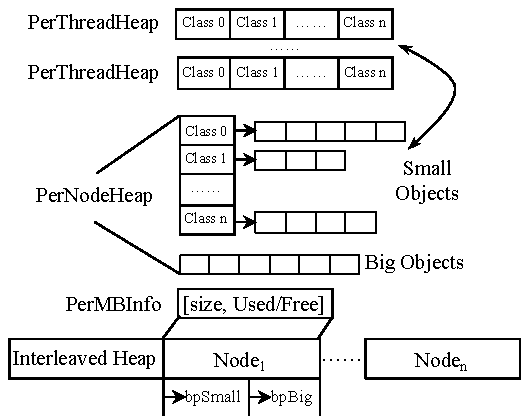
\includegraphics[width=0.45\textwidth]{figure/heaplayout1}
%\includegraphics{figure/overview2}
\end{center}
%\vspace{-0.1in}
\caption{Overview of \NA{}'s Heap Layout.
\label{fig:overview}}
%\vspace{-0.1in}
\end{figure}

As discussed in Section~\ref{sec:intro}, \NM{} proposes an origin-based memory management that should check the origin of every object upon deallocation. In order to support fast checking, \NM{}'s heap layout is designed as  Figure~\ref{fig:overview}. \NM{} requests a large and continuous block of memory from the underlying OS initially, and then divides it evenly into multiple regions based on the number of hardware nodes. Each region is bound to a different physical node via \texttt{mbind} system call. In particular, the first region is bound to the first node, the second one is bound to the second node, and so on. This design enables to compute the physical node quickly from a memory address: we could compute the index of physical node by dividing the heap offset by the region size. This layout is different from existing allocators, based on our knowledge. 

%\NM{} borrows some of these existing mechanisms. First, it uses different mechanisms to manage small and big objects. Second, small objects are also managed by size classes using the BiBOP-style. Third, similar to existing work, such as Linux and TCMalloc~\citep{tcmalloc}, \NA{} utilizes different freelists to track freed objects, and uses the first word of freed objects to link different objects. But the difference of \NM{} is further described in Section~\ref{sec:implement}.

\NM{} also manages small and big objects differently, which is similar to existing allocators as discussed in Section~\ref{sec:commondesign}. Small objects are organized by size classes, and each request will be satisfied from a particular size class. \NA{} utilizes fine-grained size classes for small objects, such as 16 bytes apart for objects less than 128 bytes, and 32 bytes apart for objects between 128 bytes and 256 bytes, then power-of-2 sizes afterwards. In \NM{}'s design, big objects are those ones with the size larger than 512K, which are typically aligned up to megabytes. As shown as Figure~\ref{fig:overview}, each per-node region will be further divided into two sub-regions, one for small objects, and one for big objects. The \texttt{pbSmall} pointer is utilized to track never-allocated small objects, and big ones are tracked with \texttt{pbBig} pointer. 

For small objects, \NM{} utilizes the well-known  ``\textbf{Bi}g-\textbf{B}ag-\textbf{o}f-\textbf{P}ages'' (BiBOP) style that all objects in the same bag (1 MB by default) will have the same size class. Big objects will be always aligned to 1MB. In order to improve the reliability~\citep{FreeGuard, Guarder}, \NM{} tracks the size information and availability information in a separate area (shown as ``PerMBInfo'' of Figure~\ref{fig:overview}): it tracks the size of each size class for small objects, and the size of the big object (aligned to 1 MB) for big objects. This data structure also includes the used/free information for big objects, which allows to coalesce multiple continuous big objects into a bigger object upon deallocations. To save space, \NM{} utilizes its lowest significant bit to encode the availability information.

Typically freed objects of the same size class will be tracked with freelists. In order to further reduce the contention, \NM{} employs per-thread heap that maintains a freelist for each size class, which requires no protection since each thread has its own per-thread heap. However, this may introduce memory blowup, as addressed in Section~\ref{sec: others}. 

In order to support the NUMA architecture, a PerNodeHeap is proposed that has one freelist for each size class and one common freelist to track all freed big objects allocated from the current node. We will talk about the relationship between per-thread freelist and per-node freelist in Section~\ref{sec:origin}. 

Overall, \NM{} includes a novel layout to quickly compute the physical node (with the memory binding) and a per-node heap to support node-aware allocations. This design allows it to perform origin-based memory management efficiently, as discussed in the next Section. 
%mechanisms to re and one per-node freelist for each node to track big objects. \NM{} also maintains per-node freelists to track small objects based on size classes. These freelists are singly linked lists, which uses the first word of every freed object as pointers.  Small freed objects may be migrated between per-thread freelists and per-node freelists, as further described in Section~\ref{sec: others}. 

\subsection{Origin-Based Memory Management} 
\label{sec:origin}

As described in Section~\ref{sec:overview}, \NM{} includes an origin-computable design that could quickly determine the origin of each object via the computation. On top of it, we further discuss other aspects of \NM{}'s origin-based memory management as follows.  

First, it includes an origin-based deallocation that will always return a freed object to a freelist with the same origin. In particular, if a freed object is originated from a different node, it is returned to its originated node's freelist. Otherwise, a small object is returned back to the thread's freelist and a big object is returned back to the current node's freelist. Comparing to node-based freelist, there is no need to acquire a lock when using the per-thread freelist. \NM{} is  different with all existing work that a freed object will be \textit{only} returned into the per-thread list if the object is originated from the current node. That is, \NM{} considers the originality of objects for deallocations.   

Second, \NM{} always ensures node-local memory allocations. For small objects, it follows this order: the per-thread's freelist will be checked first, since there is no need to acquire any lock and there is a high chance that the object is still hot in the cache; The current node's freelist will be checked secondly; The last step is to allocate the memory from the current node's un-allocated region, if the previous two steps failed. Since the region is bound to the current node, and objects in the per-thread freelist and the per-node freelist are always originated from the current node, \NM{} ensures local allocations. For big objects, allocation will be satisfied from    per-node freelists or un-allocated region (pbBig pointer) of the current node. 

\subsection{Reducing Node Imbalance}
\label{sec:balance}

\NM{} further proposes two additional mechanisms to reduce node imbalance, where it is the first to implement these mechanisms inside the memory allocator. 

\subsubsection{Interleaved Heap} 
\NA{} proposes an interleaved heap that is inspired by existing profilers\citep{XULIU, MemProf}: most NUMA performances issues  are related to shared objects allocated in the main thread. Due to the default first-touch policy~\citep{lameter2013numa, diener2015locality}, objects allocated and touched by the main thread are typically allocated in the first node that the main thread is running on. But these objects can be passed to multiple child threads, causing the load imbalance issue: the memory controller of this node will be concurrently accessed by multiple threads, leading to the performance bottleneck on this node. To overcome this issue, \NA{} reserves a range of memory for such objects, called as ``Interleaved Heap'' in Figure~\ref{fig:overview}. \NA{} utilizes the \texttt{mbind} system call to specify that physical pages of this heap will be allocated from all nodes interleavedly. With this design, then all threads can access shared objects allocated in the main thread concurrently, reducing interconnect congestion and load imbalance of a single node. 

\begin{comment}
\begin{wrapfigure}{r}{0.6\textwidth}
\centering
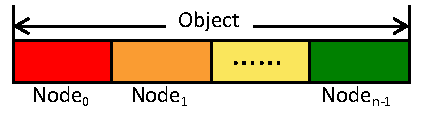
\includegraphics[width=3in]{figure/blockwise}
\vspace{-0.1in}
\caption{Block-wise Memory Allocation\label{fig:blockwise}}
\vspace{-0.1in}
\end{wrapfigure}
\end{comment}

However, \NA{} should not allocate private objects of the first thread from the interleaved heap, since that will create remote accesses unnecessarily. To achieve this, \NM{} further  differentiates shared objects from private objects. Although programmers could provide such information, that will require the change of programs or manual intervention. Instead, \NM{} utilizes a simple heuristics to identify potentially-shared objects based on allocation callsites: each allocation callsite is treated as a shared one initially, and is allocated from the interleaved heap; Whenever an object is deallocated before creating children threads, indicating such an object is a private one for the main thread,  all objects from the corresponding callsite are considered to be private ones, and then are only allocated from the per-node heap afterward. 

\NM{} monitors allocation/deallocation pattern to identify the share-ability of each callsite. If an allocation callsite is found to be private, then all allocations from this callsite should not allocate from the interleaved heap, but from the normal heap. Therefore, a challenge is to obtain and compare the callsite of each allocation so that we could determine the heap based on the share-ability. In fact, this may introduce high overhead for applications with large amount of allocations, if using the \texttt{backtrace}~\citep{DBLP:conf/icse/SumnerZWZ10, DBLP:conf/cgo/ZengR0AJ014}. For the performance reason, \NA{} utilizes the sum of the stack position and the return address of the allocation invocation to identify a callsite, called ``\textit{callsite key}''. This combination is able to differentiate callsites correctly if an application does not have allocation wrappers, since stack positions can be utilized to identify the number of functions in the stack and the return address tells the invocation placement inside the same function. If a callsite is misidentified, it will not cause any correctness issue, but with some performance penalties/losses. For the performance reason, \NA{} utilizes a hash table to track the status of every callsite. 
 % which is fortunately not very expensive given the limited amount of different callsites. 
 
Note that the interleaved heap cannot be achieved by using existing NUMA utilities like \texttt{numactl}. Although \texttt{numactl} could also specify memory allocations to be interleaved. But \texttt{numactl} could only set the policy for a whole application. Instead, \NM{} only utilizes the interleaved heap for shared objects that are allocated in the main thread, with its fine-grained memory management. As we evaluated in Section~\ref{sec:interleavedheap}, the interleaved heap is beneficial to the performance for most applications, but not all applications.  Therefore, it is better that the interleaved heap is enabled whenever necessary. 

\subsubsection{Node-Balanced Thread Binding} 
As described in Section~\ref{sec:intro}, thread migration will cause multiple performance issues for the NUMA architecture. Therefore, \NM{} binds each thread to a node specifically in order to avoid thread migration cross different nodes. To improve the balance, \NM{} binds threads to different nodes in an interleaved way so that every node will have a similar number of threads. The first thread will be bound to the node that it is scheduled to run by the OS, and the second thread will be bound to its next node, and so on. Note that \NM{} only binds a thread to a node, instead of a core, which still allows the scheduling initiated by the OS. To perform the binding correctly, \NM{} obtains the hardware topology in the initialization phase via the \texttt{numa\_node\_to\_cpus} API, which tells the relationship between each CPU core and each memory node. Then it intercepts all thread creations in order to bind a newly-created thread to a specific node. In the future, we plan to support user-controlled binding.


 
\begin{comment}
\subsection{Selective Huge Pages} 
\label{sec:hugepage}

 Based on the existing study~\citep{hugepages}, huge pages can reduce Translation Look-aside Buffer (TLB) misses, and reduce the interferences on the cache utilization caused by TLB misses, since the same size of TLB entries will cover a larger space of memory. However, existing transparent huge page support is not good for the performance~\citep{Gaud:2014:LPM:2643634.2643659, DBLP:conf/asplos/PanwarBG19}, due to hot page effect, page-level false sharing, and increased memory footprint~\citep{DBLP:conf/asplos/MaasAIJMR20}.
 
\NM{} proposes explicit huge pages to avoid these issues that could always benefit the performance based on our evaluation in Section~\ref{sec:hugepage}. The basic idea of \NM{} is to carefully choose which objects that should be allocated from huge pages: first, shared objects should not be allocated from huge pages, which may introduce page-level false sharing that multiple threads are accessing the same huge page. This will cause unnecessary load imbalance due to concurrent accesses, and remote accesses. Second, if we only utilize partial memory in the same huge pages, then we may waste the remaining memory in the same page. This problem will become more serious for \NM{}'s design, since it is using a big bag (1MB) to hold objects with the same size. 

%If huge pages are only utilized for private objects for threads running on the node, then there is no hot page effect and page-level false sharing. Also, if huge pages are only utilized for big objects that are larger than the page size, then there is no need to worry about unnecessary memory consumption. 
Based on these observations,  \NM{} only employs huge pages for large objects, with the size larger than 512KB. This design will reduce unnecessary memory waste that only partial pages are actually allocated. Also, \NM{} only employs huge pages for small objects that are predicted to be allocated frequently. For the latter one, \NM{} employs the history information to predict, and only uses huge pages for a size class that has used at least one bag before. Based on our evaluation in Section~\ref{sec:hugepage}, this design balances the performance and memory consumption, which always benefiting the performance. 

%In addition to large objects that has the size larger than the size of a huge page, huge pages are only utilized for small objects that are predicted to be used a lot.  \NA{} employs the history of memory allocation to predict this. 
%Each per-node heap is further divided into two parts as illustrated in Figure~\ref{fig:overview}: small objects will be allocated from the first half and will be allocated using small pages, while big objects will be allocated from the second half with huge pages (2MB). When a big object (with the huge page) is utilized for small objects, only frequently-allocated small objects can utilize such an object. We believe that our design balances the performance and memory consumption.   

\end{comment}

\subsection{Other Mechanisms}
\label{sec: others}

\NM{} also implements the following mechanisms in order to reduce the performance and memory overhead. 

\paragraph{Efficient Object Migration} It is important to reduce memory blowup that freed objects by one thread cannot be utilized by other ones~\citep{Hoard}.  \NM{} should move freed objects between per-thread and per-node freelists frequently. On the one hand, when a per-thread freelist has too many freed objects, some of them should be moved to the per-node freelist so that other threads could re-utilize these freed objects. On the other hand, each per-thread list needs to obtain freed objects from its per-node heap, when a thread is running out of the memory. 
Therefore, an efficient mechanism is required to support frequent migration. 

A straightforward method is to traverse the freelist to collect a specified number objects, and then moves all of them at a time in order to reduce the synchronization overhead. Both TCMalloc and TCMalloc-NUMA utilize this mechanism, which have the following issues. First, traversing the freed objects of a freelist will actually bring the first lines of these objects to the cache, since the first word of each freed object is used as the pointer for the freelist. This traverse will pollute the cache of the current thread, especially when a thread is moving these objects out. 
%\NM{} utilizes the first word of each freed object as the pointers for the linked list, where traversing these objects will bring these objects to the cache that the current thread do not need. 
Second, the migration will always migrate recently-freed objects that since they are located in the header of the list. However, this is not good for the performance when moving objects from a per-thread freelist to the per-node freelist, since recently-freed objects can be still hot in the cache. Then a thread will be forced to utilize objects that are not in the cache. 
Third, the traverse of a global freelist may introduce significant lock contention, when multiple threads are migrating freed objects from the per-node freelist concurrently.
Some applications have been observed  20\% slowdown due to this straightforward mechanism. \NM{} further proposes an efficient mechanism to migrate objects efficiently. 

\begin{figure}[!h]
\centering
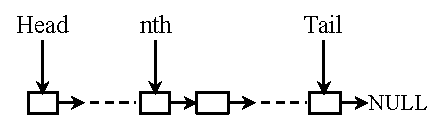
\includegraphics[width=3in]{figure/perthreadlist}
%\vspace{-0.1in}
\caption{Avoiding the traverse of per-thread freelist\label{fig:perthreadlist}}
%\vspace{-0.1in}
\end{figure}

\NM{} proposes special data structures to avoid these issues. First, each per-thread freelist maintains two pointers that pointing to the least recently-used object (shown as the \texttt{Tail} pointer) and the $nth$ object separately (shown as $nth$), as shown in Figure~\ref{fig:perthreadlist}. Each freelist has a header pointer pointing to the most recently-used object, shown as \texttt{Header}, which will be updated upon adding or deleting an object. This structure avoids the traverse of freelist during the migration, and allows the movement of the least-freed objects (between $(n+1)th$ and $Tail$) to the per-node freelist. After the migration, the \texttt{Tail} pointer will be set to the original $nth$ object. 

%\Maintaining the pointer to the $nth$ object requires only a forward traverse to obtain the pointer of $(n-1)th$ object, and then a thread can migrate $n$ objects (between $(n-1)th$ and the \texttt{Tail} object) easily. 
%After the migration,  the \texttt{Tail} pointer can be set to the original $nth$ object. However, this mechanism alone cannot reduce the lock contention when multiple threads are concurrently obtaining objects.

\begin{figure}[!ht]
\centering
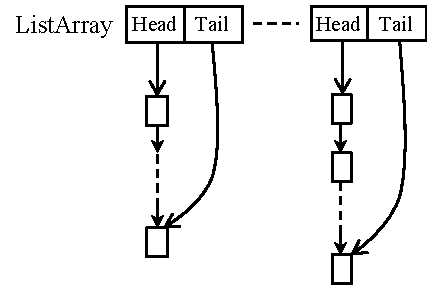
\includegraphics[width=3in]{figure/listarray}
\caption{An array of freelists for per-node heap\label{fig:listarray}}
%\vspace{-0.1in}
\end{figure}

Second, \NM{} also proposes a circular array as shown in Figure~\ref{fig:listarray} for the per-node freelist. The per-node freelist could easily become the performance bottleneck, since many threads may compete for it when they need to move objects from per-node freelist. To address this issue, each per-node freelist is actually consisted of many sub-lists, where a \texttt{Head} pointer and a \texttt{Tail} pointer point to the header and the tail of each sub-list. Then whenever a thread is migrated object  
Each per-node freelist has three types of operations that can be greatly reduced with this data structure. First, a remote thread will put a freed object into the freelist, based on the origin-based deallocation. This operation can be done in a constant time, by putting the object into the entry pointed by a \texttt{toPut} pointer. Second, a local thread maybe put multiple objects into it, which can be finished in constant time as well. All objects will be putted to the entry pointed by a \texttt{toPut} pointer, and then the pointer will be updated to the next entry. Third, the operations for getting objects from it can be done efficiently by simply moving all objects in the current entry, since there is no need to traverse the freelist. Therefore, this data structure reduces the synchronization issue of all operations. 
%In order to support the put and get operations to the freelist, this array has two pointers, \texttt{toGetIndex} and  \texttt{toPutIndex}. If a thread tries to obtain freed objects from the per-node heap, it will obtain all  objects pointed by the \texttt{toGetIndex}, and increment the index afterward. If the freelist pointed by the \texttt{toGetIndex} has no freed objects, there is no freed objects in the per-node freelist for this size class.  The put operation will utilize the pointer \texttt{toPutIndex}. There are two scenarios for the put operation. 
%First, a thread may put an freed object directly to the per-node freelist, if this object is originated from a different node that the thread does not belong to. In this case, the object will be placed into the freelist pointed by the \texttt{toPutIndex}, but the index is not updated after the deallocation. Second, when freed objects in a per-thread freelist is above the predefined watermark, the thread will migrate a batch of objects to the freelist pointed by the \texttt{toPutIndex}. After this migration, the current freelist is considered to be full, and will update the index to the next entry in the circular array.

\paragraph{Node-Local Metadata} \NM{} guarantees that all of the metadata is always allocated in the same node, based on its thread binding as described in Section~\ref{sec:balance}. Such metadata includes per-node and per-thread freelists for different size classes, and freelists for big objects. Similarly, \NM{} utilizes the \texttt{mbind} system call to bind the memory to a specific node.  

%\paragraph{Reducing Memory Waste} \NM{} utilizes multiple mechanisms to reduce memory wastes. First, if a thread exits, then all memory will be utilized by a new thread. Second, \NM{} reduces memory wastes when transparent huge pages are employed.  Multiple threads in the same node will share the same bag (for the same size class), instead of having a separate bag for each thread.  That is, when  a thread is running out of the memory, it obtains multiple objects at a time from the corresponding bag, typically in a granularity of a small page, instead of getting a new bag. Based on our evaluation, this mechanism reduces most of memory consumption, with the transparent huge page support by default.  

 %every thread has its own freelists for each size class so that there is no need to acquire the lock when an allocation can be satisfied from its per-thread heap, similar to TCMalloc. That is, two threads will not share the same per-thread heap. However, some applications may create new threads after some threads have exited. \NM{} re-utilizes the memory for these exited threads. Basically, \NM{} intercepts thread joins and cancels so that it can assign heaps of exited threads for newly-created threads, and re-utilize their heaps correspondingly.  


%\paragraph{Transparent Huge Page Support:} During the development, we noticed that excessive memory consumption can be imposed when the OS enables transparent huge pages by default. In order to reduce memory consumption, \NM{} makes multiple threads share the same bag (for the same size class), instead of having a separate bag for each thread. If each thread is running out of the memory, it obtains multiple objects at a time from the corresponding bag. Currently, if a class size is less than one page, then we will at most get objects with the total size of one normal page. Otherwise, it will get 4 objects (with the size less than 64 KB) or 2 objects afterward. Based on our evaluation, this mechanism actually reduces the memory consumption for multiple times for a machine with 128 cores and 8 nodes, with the transparent huge page support by default.  

%\paragraph{Cache Warmup} \NM{} also borrows the cache warmup mechanism of TCMalloc~\citep{tcmalloc}: it will insert all objects in a page into the freelists, if there is no objects in the per-thread freelist. We believe that inserting multiple objects into the freelist will benefit data prefetches, since the insertion is a simple and predictable pattern. With this mechanism, \texttt{raytrace} improves the performance by 10\%. However, this is the only application that we observed such performance improvement. There is no impact on other applications. 

%TCMalloc utilizes a \texttt{mmap} system call to obtain multiple pages (depending on the class size) from the OS each time, when it is running out of the memory for one size class. For such a memory block, TCMalloc inserts all objects of this block into its central freelist at one time. Since TCMalloc utilizes the first word of each object as the pointer for the freelist, this mechanism warms up the cache by referencing the first word of each object during the insertion. According to our observation, this warmup mechanism improves the performance of one application (\texttt{raytrace}) by 10\%. Based on our understanding, the performance improvement is caused by data prefetches, since inserting objects to the freelist has a simple and predictable pattern. \NM{} employs a similar mechanism for small objects with the size less than 256 bytes, and adds all objects inside a page to the per-thread freelist. 

%we propose the combination of per-node heap and per-thread cache. In order to reduce the contention, \NM{} will obtain multiple objects at a time from the per-node heap. 

 
%https://queue.acm.org/detail.cfm?id=2852078

